\section{(Auto-)Mobile Society}

\subsection{Einführung: Vom Industrie- zum Konsumzeitalter}

Die Vorlesung untersucht die gesellschaftlichen Veränderungen,
die sich in der zweiten Hälfte des 20. Jahrhunderts vollziehen.

Im Mittelpunkt steht dabei das Automobil,
das nicht nur ein technisches Artefakt,
sondern auch ein Symbol moderner Mobilität,
individueller Freiheit und gesellschaftlichen Wandels darstellt.

Die Vorlesung knüpft an die vorherige Sitzung über Eisenbahn und Taktfahrplan an.

Während dort die Entwicklung öffentlicher Verkehrsinfrastrukturen im Zentrum stand,
rückt nun der Individualverkehr in den Fokus.

Zentrale Leitfragen:

\begin{itemize}
    \item Wie wurde das Automobil zum Massenkonsumgut?
    \item Welche gesellschaftlichen Veränderungen ermöglichte die Massenmotorisierung?
    \item Wie hängen Mobilität, Konsum und industrielle Produktion zusammen?
    \item Welche Formen von Kontrolle und Disziplinierung stehen hinter individueller Freiheit?
\end{itemize}

Die Geschichte des Automobils ist daher nicht nur Technikgeschichte,
sondern auch Konsum-, Sozial- und Kulturgeschichte.

\subsection{Massenmotorisierung und individuelle Freiheit}

Die breite Verfügbarkeit des Automobils setzte in den USA bereits
vor dem Zweiten Weltkrieg ein.

In Europa entwickelte sich die Massenmotorisierung
vor allem nach 1945.

Das Auto wurde zum Symbol persönlicher Freiheit.

Neue Möglichkeiten entstanden für:

\begin{itemize}
    \item Freizeit und Tourismus
    \item Ausflüge und Reisen
    \item räumliche Unabhängigkeit
    \item individuelle Lebensgestaltung
\end{itemize}

Mobilität wurde zunehmend als selbstverständlicher Bestandteil
des modernen Lebens verstanden.

\begin{center}
    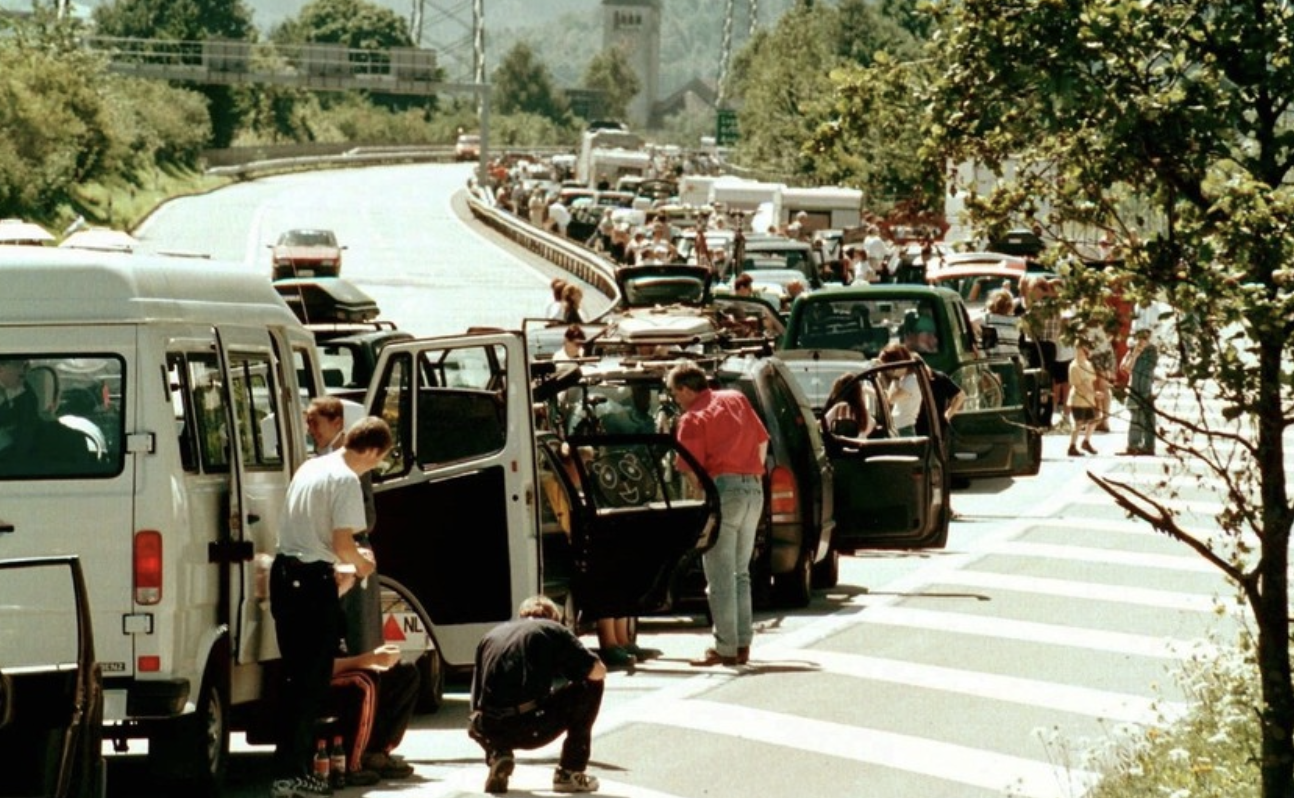
\includegraphics[width=0.75\linewidth]{images/gotthard_stau.png}
\end{center}

\subsection{Automobilisierung und neue Lebensformen}

Die Ausbreitung des Automobils veränderte nicht nur den Verkehr,
sondern auch die Siedlungsstrukturen.

Mit der zunehmenden Verbreitung von Autos entstanden Vororte
und neue Wohnformen ausserhalb der Stadtzentren.

Kennzeichnend waren:

\begin{itemize}
    \item Suburbanisierung
    \item Ausbau des Strassennetzes
    \item räumliche Trennung von Wohnen und Arbeiten
    \item Orientierung am bürgerlichen Lebensstil
\end{itemize}

Die moderne Mobilität veränderte dadurch ganze Landschaften
und prägte den Alltag breiter Bevölkerungsschichten.

\begin{center}
    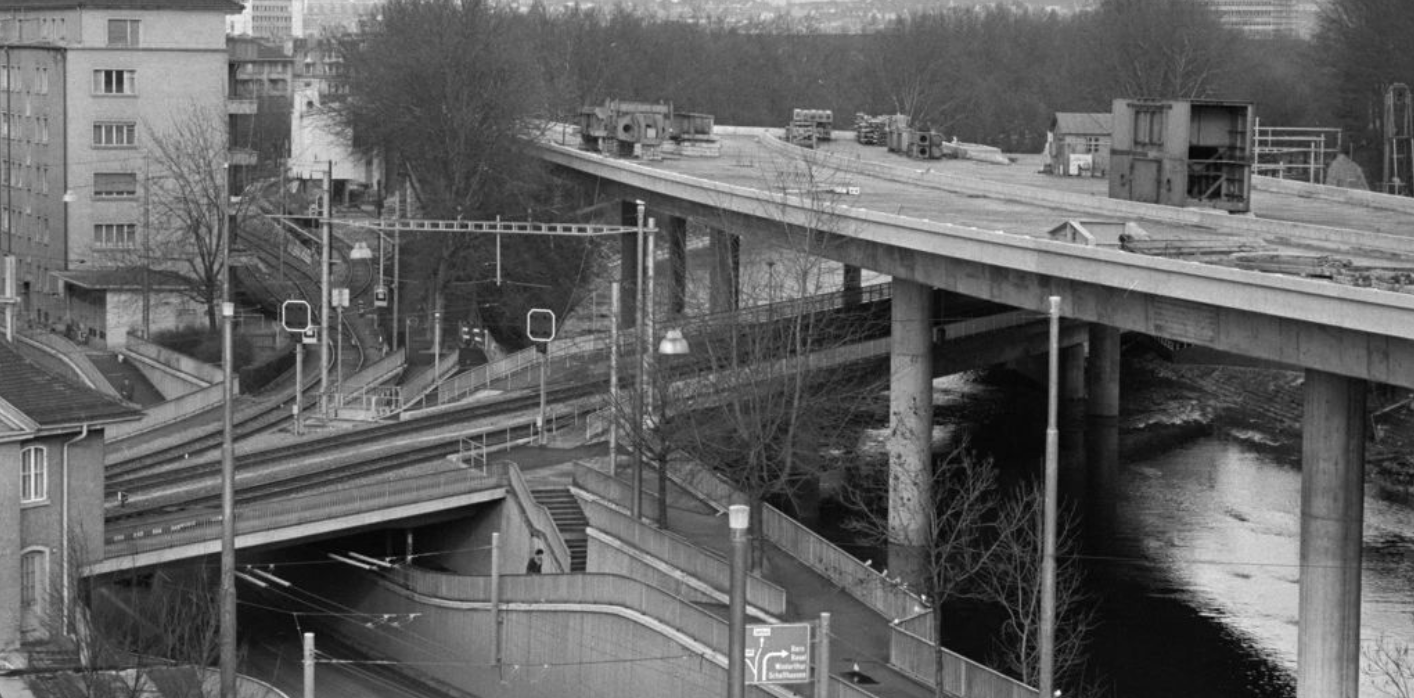
\includegraphics[width=0.8\linewidth]{images/suburbia_autobahn.png}
\end{center}

\subsection{Die frühen Konflikte des Automobils}

Die Einführung des Automobils verlief keineswegs konfliktfrei.

Zu Beginn des 20. Jahrhunderts konkurrierte das Auto
mit etablierten Verkehrsmitteln wie dem Fahrrad,
dem Fussverkehr und dem Pferdeverkehr.

Kritisiert wurden insbesondere:

\begin{itemize}
    \item Lärm
    \item Staubentwicklung
    \item Unfallgefahren
    \item Eingriffe in bestehende Verkehrsordnungen
\end{itemize}

Die Geschichte des Automobils zeigt,
dass technische Innovationen häufig gesellschaftliche Aushandlungsprozesse auslösen.

\begin{center}
    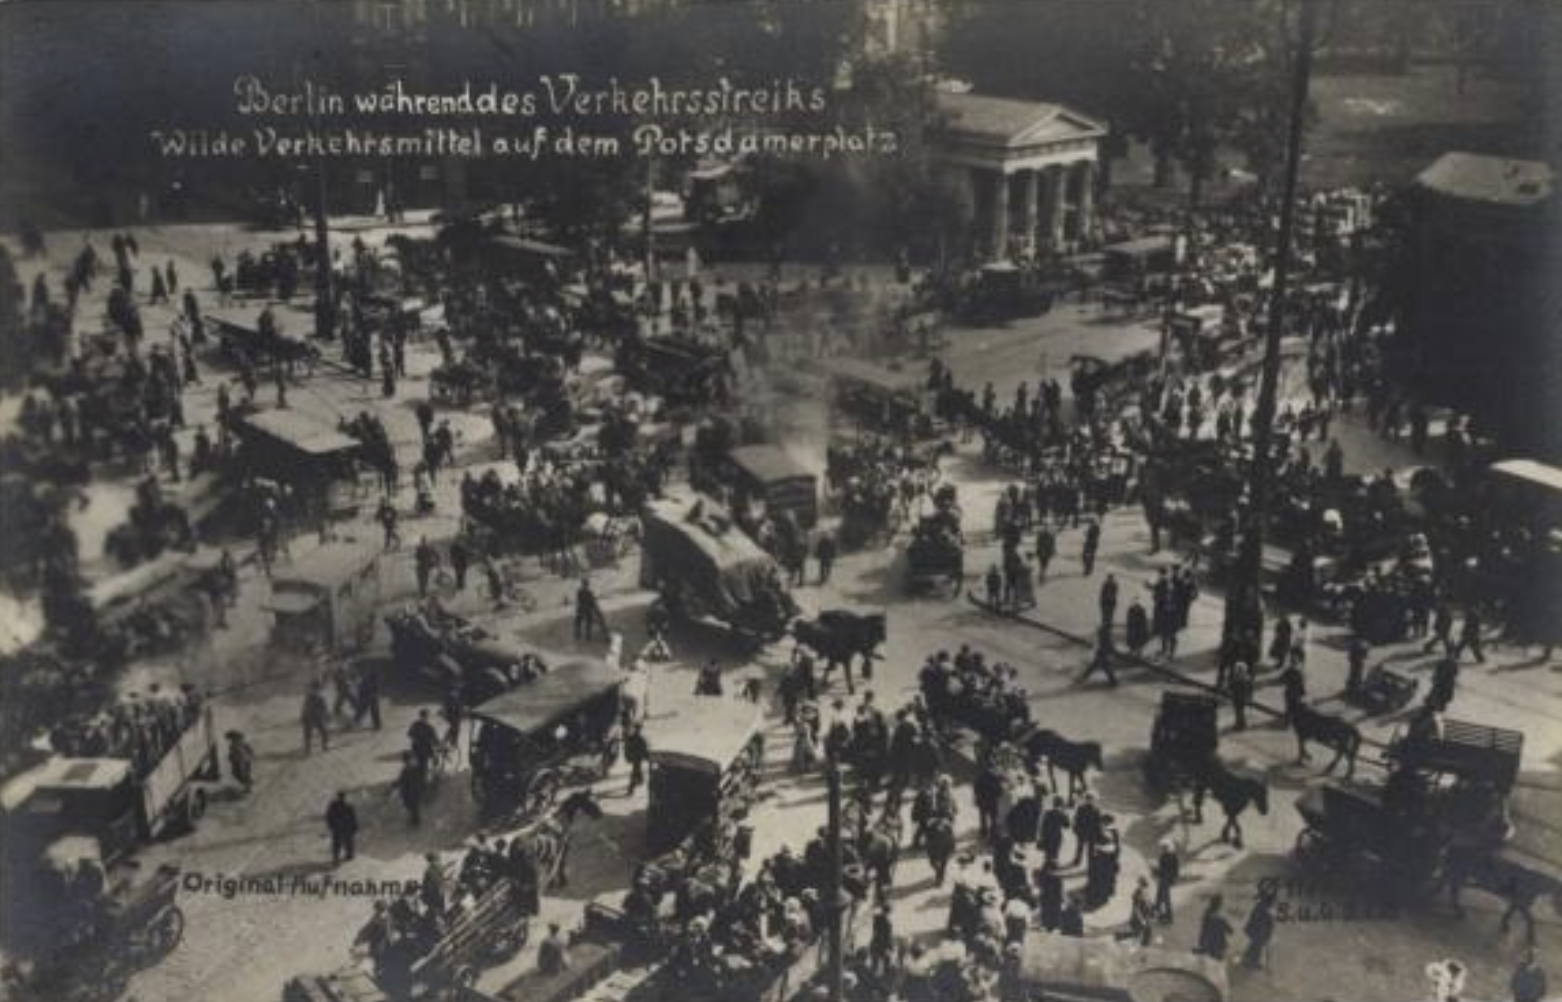
\includegraphics[width=0.75\linewidth]{images/potsdamerplatz_1921.png}
\end{center}

\subsection{Das Auto als Symbol von Geschwindigkeit und Individualismus}

Schon früh wurde das Automobil nicht nur als Transportmittel,
sondern auch als Freizeit- und Sportgerät inszeniert.

Autorennen erfüllten mehrere Funktionen:

\begin{itemize}
    \item Erprobung neuer Technologien
    \item Werbung für Hersteller
    \item Inszenierung technischer Leistungsfähigkeit
    \item Vermarktung von Geschwindigkeit und Freiheit
\end{itemize}

Dadurch entstand das bis heute wirksame Bild des Autos
als Ausdruck von Individualität und persönlicher Unabhängigkeit.

\begin{center}
    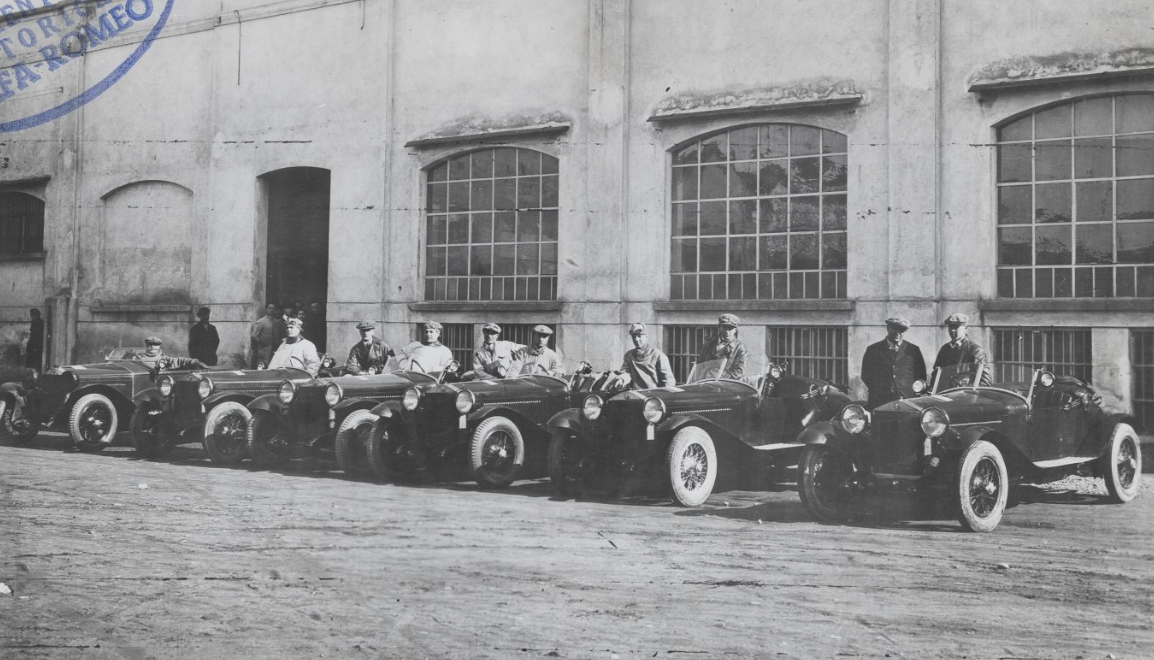
\includegraphics[width=0.75\linewidth]{images/autorennen_fruehes_20jh.png}
\end{center}

\subsection{Vom Industrieprodukt zum Konsumgut}

Die Vorlesung stellt die Frage,
wie das Automobil vom Luxusobjekt zum Massenprodukt werden konnte.

Der Schlüssel liegt in der Entwicklung neuer Produktionsformen.

Technische Innovationen allein genügten nicht.

Entscheidend waren neue Organisationsformen der Arbeit,
die eine kostengünstige Massenproduktion ermöglichten.

\subsection{Taylorismus und wissenschaftliche Arbeitsorganisation}

Ende des 19. Jahrhunderts entwickelte Frederick Winslow Taylor
das Konzept des Scientific Management.

Ziel war die wissenschaftliche Optimierung industrieller Arbeit.

Kennzeichnend waren:

\begin{itemize}
    \item Zerlegung komplexer Tätigkeiten in Einzelschritte
    \item Standardisierung von Arbeitsabläufen
    \item Zeitmessung mit Stoppuhren
    \item Trennung von Planung und Ausführung
    \item Kontrolle der Arbeitsleistung
\end{itemize}

Der Taylorismus bildete eine wichtige Grundlage
für die spätere Massenproduktion.

\subsection{Die Bewegungsstudien der Gilbreths}

Frank und Lillian Gilbreth erweiterten den Taylorismus
durch die systematische Analyse menschlicher Bewegungen.

Mithilfe von Fotografie und sogenannten Chronocyclegraphs
wurden einzelne Handgriffe sichtbar gemacht.

Ziel war die Reduktion unnötiger Bewegungen
und die weitere Steigerung der Effizienz.

Der menschliche Körper wurde damit selbst
zum Gegenstand technischer Optimierung.

\begin{center}
    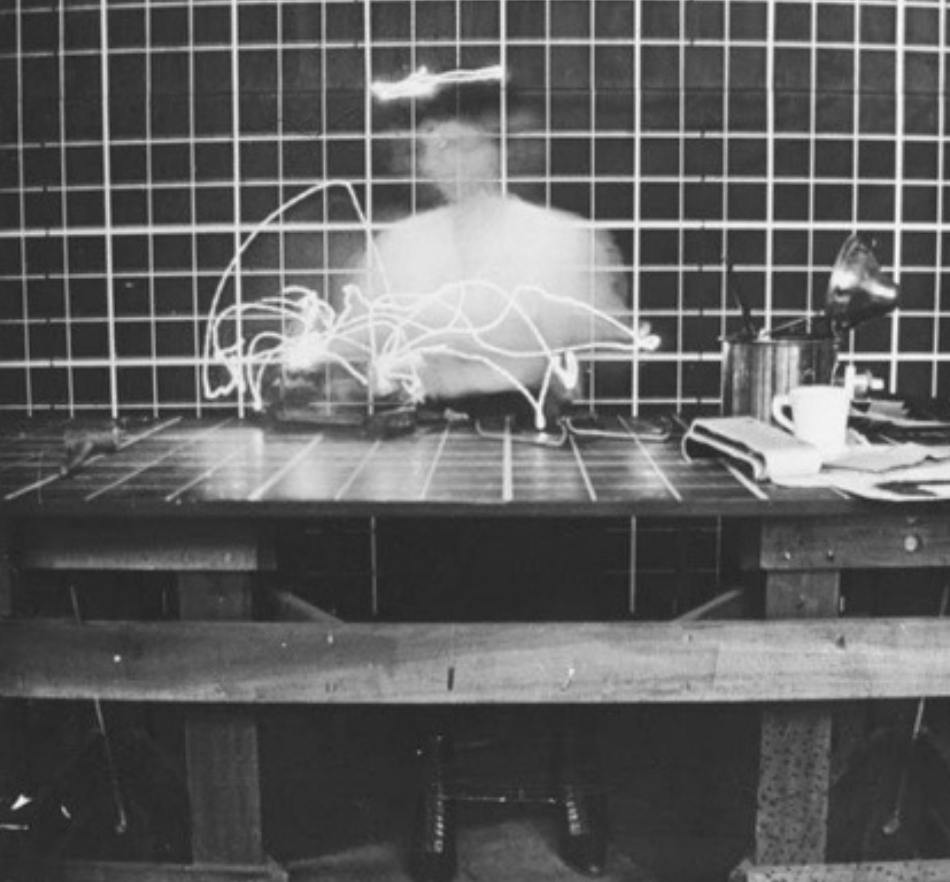
\includegraphics[width=0.7\linewidth]{images/gilbreth_studie.png}
\end{center}

\subsection{Fordismus und Fliessbandproduktion}

Mit Henry Ford erreichte die Rationalisierung industrieller Arbeit
eine neue Stufe.

Ab 1913 wurde die Automobilproduktion
durch das Fliessband grundlegend verändert.

Merkmale des Fordismus:

\begin{itemize}
    \item kontinuierliche Massenfertigung
    \item standardisierte Arbeitsschritte
    \item hohe Produktionszahlen
    \item sinkende Produktionskosten
    \item Taktung der Arbeit durch Maschinen
\end{itemize}

Die Geschwindigkeit der Maschinen bestimmte nun den Arbeitsrhythmus der Beschäftigten.

Dadurch wurde das Automobil erstmals für breite Bevölkerungsschichten erschwinglich.

\begin{center}
    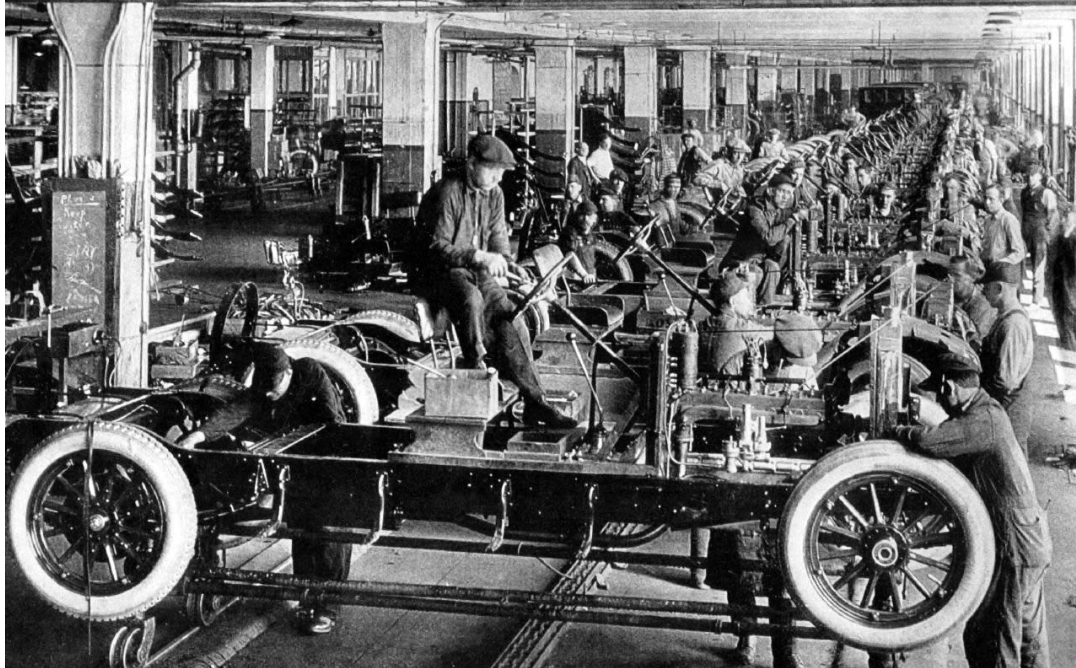
\includegraphics[width=0.8\linewidth]{images/ford_fliessband.png}
\end{center}

\subsection{Globale Rohstoffe und Fordlândia}

Die Automobilproduktion war auf globale Rohstoffketten angewiesen.

Besonders wichtig war Kautschuk für die Herstellung von Reifen.

Der weltweite Kautschukhandel beruhte vielfach
auf kolonialen Herrschaftsverhältnissen und Ausbeutung.

Henry Ford versuchte deshalb,
mit der brasilianischen Siedlung Fordlândia
eine eigene Kautschukproduktion aufzubauen.

Das Projekt scheiterte jedoch.

Die Ursachen lagen in:

\begin{itemize}
    \item fehlender Kenntnis lokaler Bedingungen
    \item ökologischen Problemen
    \item Widerstand der lokalen Bevölkerung
\end{itemize}

Die Geschichte von Fordlândia verdeutlicht,
dass technische und wirtschaftliche Modelle
nicht beliebig auf andere Gesellschaften übertragen werden können.

\begin{center}
    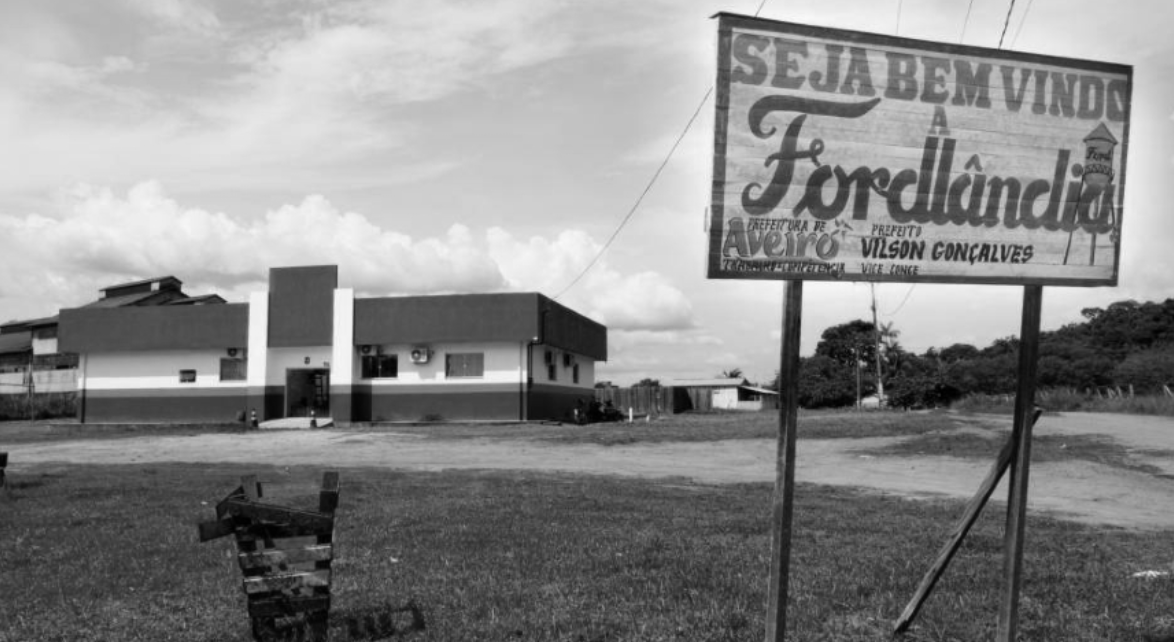
\includegraphics[width=0.75\linewidth]{images/fordlandia.png}
\end{center}

\subsection{Produzenten und Konsumenten}

Ford veränderte nicht nur die Produktion,
sondern auch die Beziehung zwischen Unternehmen und Beschäftigten.

1914 führte Ford vergleichsweise hohe Löhne
und kürzere Arbeitszeiten ein.

Ziel war es,

\begin{itemize}
    \item die Fluktuation zu reduzieren
    \item die Produktivität zu steigern
    \item Arbeiter zu Konsumenten zu machen
\end{itemize}

Gleichzeitig kontrollierte das Unternehmen
über das sogenannte Sociological Department
das Privatleben seiner Beschäftigten.

Die Entstehung der Konsumgesellschaft war damit eng
mit neuen Formen sozialer Kontrolle verbunden.

\subsection{Bewegung und Kontrolle}

Die Vorlesung endet mit einer grundlegenden Beobachtung:

Die moderne Freiheit zur individuellen Mobilität
beruht auf umfangreichen technischen,
organisatorischen und gesellschaftlichen Kontrollmechanismen.

Damit Menschen sich frei bewegen können,
müssen gleichzeitig

\begin{itemize}
    \item Arbeitsprozesse diszipliniert werden,
    \item Verkehrsinfrastrukturen organisiert werden,
    \item Landschaften umgestaltet werden,
    \item globale Lieferketten kontrolliert werden.
\end{itemize}

Mobilität und Kontrolle stehen daher nicht im Widerspruch,
sondern sind eng miteinander verbunden.

\begin{center}
    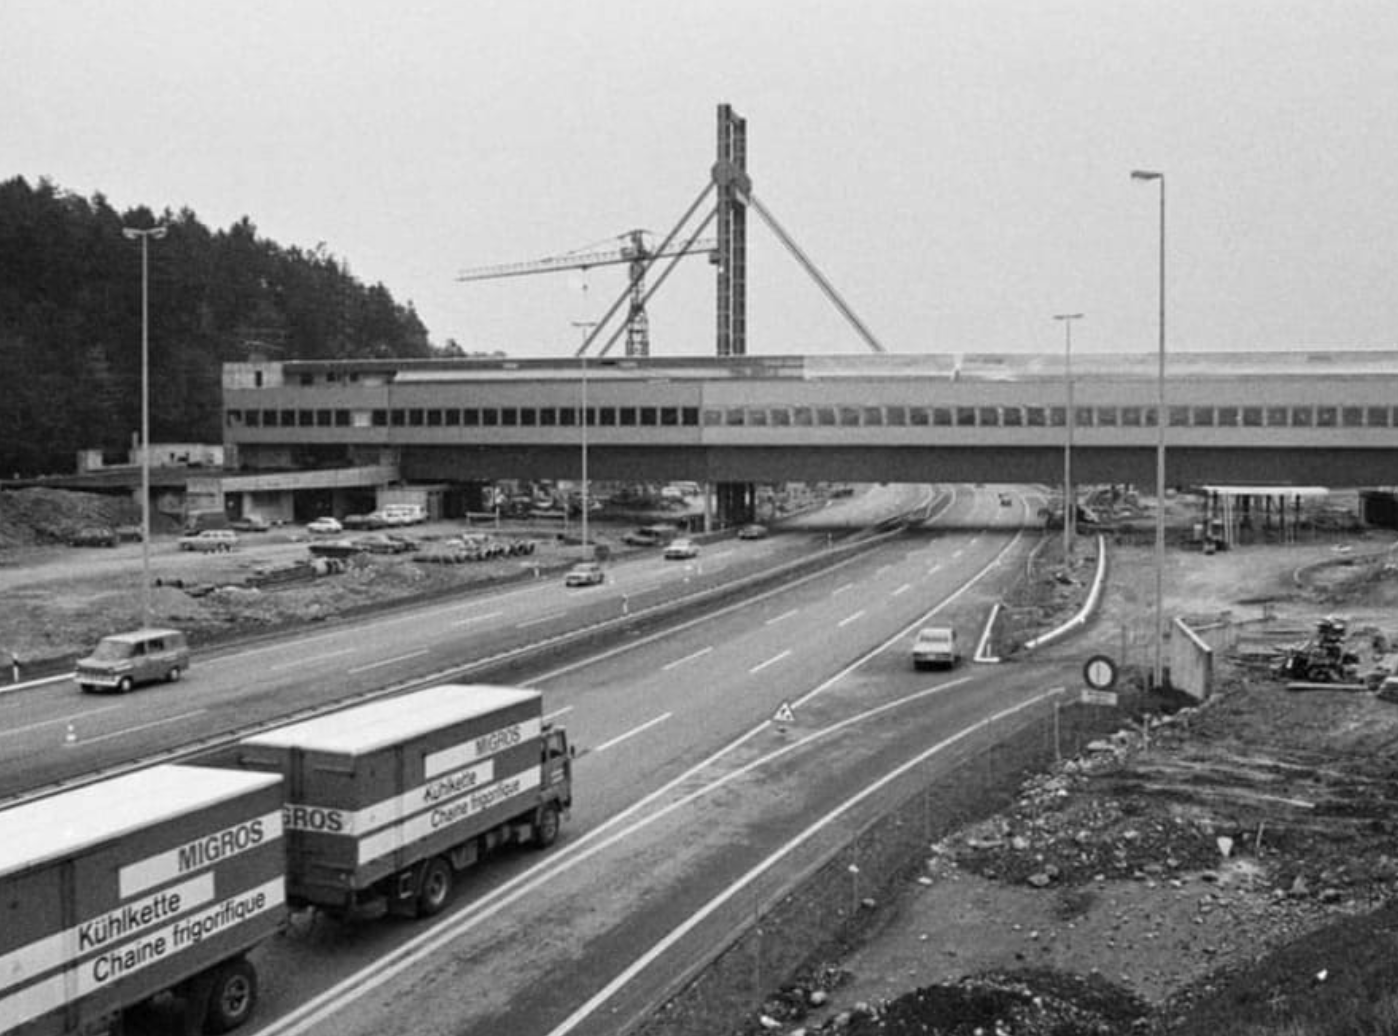
\includegraphics[width=0.8\linewidth]{images/fressbalken_wuerenlos.png}
\end{center}

\subsection{Zentrale Erkenntnisse}

Die Geschichte des Automobils ist keine reine Erfolgsgeschichte technischer Innovation.

Sie zeigt:

\begin{itemize}
    \item den Übergang von der Industrie- zur Konsumgesellschaft
    \item die Bedeutung der Massenproduktion
    \item die Verbindung von Mobilität und individueller Freiheit
    \item die globale Verflechtung industrieller Produktion
    \item die Rolle von Kontrolle und Disziplinierung in modernen Gesellschaften
\end{itemize}

Die zentrale These lautet:

Die moderne Automobilgesellschaft entstand nicht allein durch technische Erfindungen.
Sie wurde durch neue Produktionsformen,
globale Rohstoffketten,
Konsumpraktiken und gesellschaftliche Leitbilder von Freiheit ermöglicht.